%-------------------------------------------------------------------------------
% TEMPORAL DISCRETIZATION AND SOLVERS 
%-------------------------------------------------------------------------------

\section{Temporal Discretization and Solvers} \label{sec:time}

Time-stepping refers to the time integration or time discretization of
time-dependent differential equations. In the previous section, we have seen
the benefits of using a spectral discretization of the spatial dimension of our
problem. Due to its nature, the time component is usually discretized with a
local discretization, not a global discretization such as a spectral one. The
first thing to note is that time integration is affected by the resolution of
the spatial discretization of the problem. However, as mentioned, this will be
less of a problem with our pseudo-spectral approach.

The continuous time domain is divided into discrete time intervals or steps. In
this case, an equispaced grid $t_j = jh$ (where $j$ goes from $0$ to $N$) is
employed in the time domain $t \in [0, T]$, where $h$ corresponds to the time
interval for each step.

There exist various discretizations for the time operator. In an explicit time
scheme, the values of the dependent variables at a future time step are
computed solely based on the values of the dependent variable at the current
time step and previous time steps. On the contrary, an implicit time scheme
uses the values of the dependent variable of the current and future time steps.

The time-dependent equation \eqref{eq:str} is nonlinear and also classified as
a stiff equation. Stiff equations generally involve dynamics that change
rapidly on one timescale whereas slowly on another. These phenomena are
characterized by a large range of magnitude of eigenvalues associated with the
discrete problem.

Explicit time schemes become very slow for stiff equations as time step $h$ has
to be chosen very small. Otherwise, the numerical scheme will become unstable.
A stable time scheme ensures that small errors in the initial conditions or
numerical approximations do not amplify and cause the solution to become
unbounded or oscillated and will converge to the underlying function. For our
Chebyshev discretization already for the 1D case, time-stepping is stable only
if $h$ is of $O(1/N^2)$ or smaller \citep{boyd2001}.

An implicit time scheme has to be used to ensure stability and means that we
have to solve a nonlinear equation at every time step $t_j$. 

\subsection{Implicit Euler Method}

In this study, the implicit Euler method is used. The Euler method is a stiff,
stable method, and it can be characterized as the first-order backward
differentiation formula (BDF1) \citep{meseguer2020}. It is a straightforward
method and, when applicable, is used in many stiff problems.

Given an autonomous ordinary differential equation (ODE) of the form:
\begin{equation}
  \frac{{dx}}{{dt}} = f(x),
\end{equation}

where $x$ represents the dependent variable and
$f(x)$ is the derivative function with respect to $t$, the implicit Euler
approximates the solution $x_{j+1}$ of the next timestep by
\begin{equation}
  x_{j+1} = x_j + h \cdot f(x_{j+1}),
\end{equation}

where $h$ is the timestep size and $t_j$ and $x_j$ represent the time and
solution at the $j$-th timestep, respectively.

\subsection{Streamfunction Time-Stepping Equation}

Some adjustments must be made to apply the Euler method to the R4CF. First, the
one-dimensional problem naturally generalizes to problems where $\mathbf{x}$ is
a finite-dimensional vector. Secondly, the streamfunction equation involves the
Laplace operator applied to the streamfunction, which means that the time
derivative is applied to the Laplacian of the streamfunction. Overall, the time-stepping
equation reads
\begin{align}
  \Delta\Psi_{j+1} = \Delta\Psi_j + h \cdot (\frac{1}{\Rey}\Delta^2 \Psi_{j+1} +
  (\partial_x \Psi_{j+1}) \partial_y(\Delta \Psi_{j+1}) -
  (\partial_y \Psi_{j+1}) \partial_x(\Delta \Psi_{j+1})). \label{eq:str_timestepping}
\end{align}

The equation can be rewritten as follows:
\begin{align}
  F(\Psi_{j+1}) & = \Delta\Psi_j - \Delta\Psi_{j+1} + h (\frac{1}{\Rey}\Delta^2 \Psi_{j+1} +
  (\partial_x \Psi_{j+1}) \partial_y(\Delta \Psi_{j+1}) -
  (\partial_y \Psi_{j+1}) \partial_x(\Delta \Psi_{j+1})) \nonumber \\
  & =  0 \label{eq:newton_ts}
\end{align}

This means that in order to calculate the solution for the next timestep
$t_{j+1}$ from a given solution at time $t_j$, we have to solve the nonlinear
equation \eqref{eq:newton_ts}. The equation for the cavity flow is usually
solved with a Newton-Raphson algorithm \citep{kuhlmann2019}, which is briefly
introduced in the following section. 

\subsection{Newton-Raphson Method}

The Newton-Raphson algorithm is an iterative method used to find the roots of a
system of nonlinear equations. Given a system of $p$ nonlinear equations
$F(\mathbf{x}) = \mathbf{0}$, the algorithm starts with an initial guess
$\mathbf{x}_0$ and iteratively improves the solution by updating the guess
using the formula:
\begin{align} 
\mathbf{x}_{k+1} = \mathbf{x}_k - J_F(\mathbf{x}_k)^{-1} \cdot F(\mathbf{x}_k),
\end{align}

where $\mathbf{x}_{k+1}$ is the updated guess at the $(k+1)$-th iteration,
$J_F(\mathbf{x}_k)$ is the Jacobian matrix of partial derivatives of $F$
evaluated at $\mathbf{x}_k$, and $F(\mathbf{x}_k)$ is the vector of function
values evaluated at $\mathbf{x}_k$.

The algorithm continues to iterate until a convergence criterion is satisfied,
typically by checking the norm of the update $\|\mathbf{x}_{k+1} -
\mathbf{x}_k\|$ against a tolerance value.

The Newton-Raphson algorithm is known for its fast convergence when the initial
guess is sufficiently close to the solution, and the Jacobian matrix is well
conditioned.

\subsection{Preliminary Results with Time Integration}

To motivate the following section on bifurcation analysis, the logical next
step would be to use the time integration and the spectral discretization to
compute solutions of the streamfunction equation \eqref{eq:str}. It is then
interesting to see if the regularized problem will produce such asymmetric
solutions shown in figure \ref{fig:4fsc_states}. Figure \ref{fig:timestepping}
shows the time-stepping result for a Chebyshev grid of size $64 \times 64$. The
time stepper is launched at different Reynolds numbers with various random
initial values of the order of $10^{-3}$ to avoid converging to the unstable
symmetric solution.

\begin{figure}[h!]
\begin{center}
  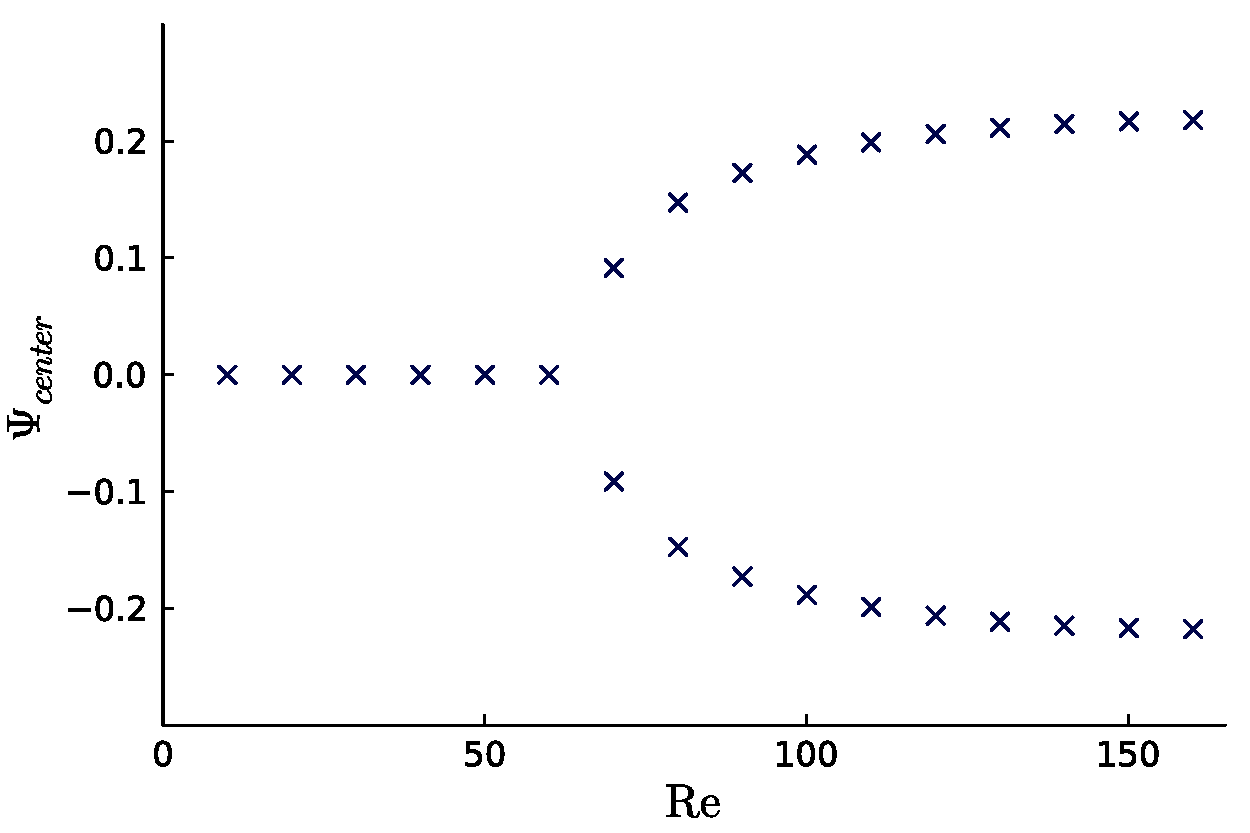
\includegraphics[width=0.59\textwidth]{figs/timestepping64x64.pdf}
\end{center}
\caption{Value of the center grid point of the streamfunction after $150$
  timesteps with $h=1$ for different Reynolds numbers up to $160$}
\label{fig:timestepping}
\end{figure}

It becomes clear that at a certain Reynolds number (around $60$), two
asymmetric branches start to emerge, which correspond to the solutions of the
non-regularized case. Furthermore, the base symmetric solutions are not
attained anymore by time evolution. To analyze these different solution types
and their stability, we will have to introduce tools of bifurcation analysis.
